% % % % % % % % % % % % % % % % % Preamble for notes % % % % % % % % % % % % % % % % % % % % % % % %
\documentclass[12pt,oneside,a4paper]{article}


% % % % % Sprogpakker og Layout % % % % % % % % %
\usepackage[left=2.5cm,top=2.0cm,bottom=1.5cm, right=3.0cm]{geometry}
\usepackage{ulem}
\usepackage[danish,english]{babel}
\usepackage[utf8]{inputenc}
\linespread{1.3}       % simulerer Word 1.5 line spacing

% % % % % % % % % % Øvrige vigtige pakker % % % % %
\usepackage{graphicx}
\graphicspath{{./Figures/}}
\usepackage{amsmath}
\usepackage{amssymb}
\usepackage{url}
\usepackage{cancel}
\usepackage{booktabs}
\usepackage{pdfpages}
\usepackage{mathpazo}
\usepackage[section]{placeins}
\usepackage{caption}
\usepackage{wrapfig}
\usepackage{tocloft}
\usepackage{subfig}
\usepackage{fancyhdr}
%Muliggør 'flere figurer i én' Eksempel på anvendelse (indenfor figure-environment):
% \subfloat[undercaption 1]{\label{label 1}\includegraphics[bredde 1]{billede 1}}
% \subfloat[undercaption 2]{\label{label 2}\includegraphics[bredde 2]{billede 2}}
% \caption{overordnetcaption}
% \label{overordnet label}
\usepackage{lscape}
%Omdanner en del af dokumentet til landscape. Angives med \begin{landscape}
\usepackage{framed}
%Sætter en ramme om et område begrænset af \begin{framed} og \end{framed}.
%Allows footnotes
\usepackage{footnote}
\setlength{\parindent}{0cm}
\setlength{\parskip}{0.3cm}
% % % % % % COMMANDS % % % % % % % %

\numberwithin{equation}{section}
\begin{document}

\selectlanguage{english}
% % % % % % % % % % % % % % % % % % % % % % Forside % % % % % % % % % % % % % % % % % % % % % % % % %
\pagenumbering{roman}

\begin{center}
{\textsc {\LARGE \bf{Københavns Universitet \\[0.3cm]  Bachelorstudiet i fysik}}}\\[1.5cm]
{\textsc {\Large \bf Førsteårsprojekt 2017}}\\[0.8cm]
{\Large Projekt nummer: 2017-06}\\[1cm]

\rule{15cm}{0.01cm}\\[1cm]
{\LARGE\bf  Bouncing ball}\\ [0.5cm]
\rule{15cm}{0.01cm}\\[1cm]
\end{center}

\vfill
{\large Forfattere:}\\
{\large \hspace*{1cm} \makebox[6cm][l]{Andreas M. Faber}  \hspace{1cm} KU- ID: \makebox[2cm][l]{QZJ517} \\
{\large \hspace*{1cm} \makebox[6cm][l]{Benjamin T. Søgaard}   \hspace{1cm} KU- ID: \makebox[2cm][l]{MGX877} \\
{\large \hspace*{1cm} \makebox[6cm][l]{Joachim J. Kønigslieb}   \hspace{1cm} KU- ID: \makebox[2cm][l]{GWC666} \\

{\large Vejledere:}\\
{\large \hspace*{1cm} \makebox[6cm][l]{Jörg Helge Müller}  \hspace{1cm} Email: \makebox[2cm][l]{muller@nbi.ku.dk} \\

\vfill

{\large Rapporten omfatter {\bf 1} siders hovedtekst og {\bf 1} siders appendix.}

{\large Rapporten er indsendt som en pdf-fil den 17 marts 2017. }

\normalsize


% % % % % % % % % % % % % % % % % % % % % % Abstract  og Indholdsfortegnelse % % % % % % % % % % % % % % % % 
\newpage
\begin{abstract}
Kort resumé, gerne på både dansk og engelsk.
\end{abstract}

\newpage

\tableofcontents


% % % % % % % % % % % % % % % % % % % % % % Indhold % % % % % % % % % % % % % % % % % % % % % % % % %
\newpage
\pagenumbering{arabic}
\section{Introduction to chaos}
\label{chaos}
As we will soon see, this experiment exhibits chaotic behavior for certain sets of parameters. Therefor it can be useful to take a moment to examine a simpler chaotic system that has many of the same qualities our experiment has. To this end, consider the simple nonlinear recurrence relation

\begin{equation}
x_{n+1}=\lambda x_n (1-x_n)
\end{equation}

This is called the logistic map, and it has some interesting attributes. If we choose $x_0$ to be between 0 and 1, and lambda to be between 0 and 3, no matter where on the interval $x_0$ starts, it seems to gravitate towards some value (dictated by $\lambda$) for increasing n. This can be visualized with a graphical procedure with which the logistic map can be easily iterated without use of a computer or calculator. First, plot the functions $f(x)=\lambda x (1-x)$ and $g(x)=x$ in the same window. Next, choose your $x_0$. Now draw a vertical line until it intercepts $f(x)$. On the y-axis, this is of course the value of $x_1$ since we took our $x_0$ and plugged it into the equation $\lambda x (1-x)$. To get $x_2$, we must now do the same we just did with $x_0$ for $x_1$. To this end we need to convert our value for $x_1$ that we have found on the y-axis to a value on the x-axis. Therefor, go to horizontally to the graph for $g(x)$. The x-coordinate of the point marks our value $x_1$, and we can now vertically return to our graph of $f(x)$ to obtain $x_2$ on the y-axis, which we convert to the x-axis by again going to $g(x)$, and so on. Through many iterations and if sweeping for $0<x_0<1$ and $0<\lambda<3$, we see that for $n\rightarrow \infty$, $x_n$ tends towards certain values, which are determined by $\lambda$, and that if $0<\lambda<1$, this value is 0. This is of course what's known as a convergent, and not not necessarily all that interesting. However, something remarkable happens if we permit lambda to be greater than 3.


\section{Model of the system}
\label{modelling}
\subsection{General model}
We will model our experiment as a 1-dimensional system that is we will not account for sideways motion. On figure \ref{bounces} two consecutive bounces can be seen where the later is bigger due to the plate  moving upwards at the time of impact.
\begin{figure}[h]
	\centering
	\includegraphics[width=0.6\textwidth]{Figures/bounceplot.eps}
	\caption{Plot of two bounces on the vibrating plate}
	\label{bounces}
\end{figure}
The $k^{\text{th}}$ bounce can be completely described by the time $t_k$ it left the plate and the velocity $v_k$ at that instance. Time and phases $\phi_k$ can be used interchangeably through the relationship $\phi=2\pi f t$.

To describe the system during a specific bounce we denote the distance of the ball above the plates rest position $y_b(t)$. Similarly we define $y_p(t)$ as the displacement of the vibrating  plate from it equilibrium. For a given frequency $f$, phase shift $\phi$ and amplitude $A$ the equation of motion for the plate is
\begin{equation}
	y_p(t)= A \cos(2\pi f t+ \phi)
	\label{platey}
\end{equation}
In air the ball is essentially a body in free fall, and since it is quite small and dense, the air resistance can be ignored. Thus the equation of motion for the ball $y_b(t)$ for the $k^\text{th}$ jump has the initial conditions $v_k$, $y_p(t_k)$ at time $t_k$, simply is
\begin{equation}
	y_{b,k}(t) = -\frac{g}{2}(t-t_k)^2+v_k(t-t_k)+y_p(t_k)
	\label{ybeq}
\end{equation}
For each jump we will denote the change of in initial $y$-coordinate\footnote{In general it is not possible to find $\Delta y_k$ analytically as it would require one to find the intersection between the graph of a parabola and a sine wave.} as $\Delta y_{k}=y_p(t_{k+1})-y_p(t_{k})$. Plugging that into (\ref{ybeq}) and solving for $t$ determines the fly time of each jump.
\begin{equation}
	\Delta t_{k} = t_{k+1}-t_{k} = \frac{v_{k}+\sqrt{v_k^2-2g\Delta y_k}}{g}
	\label{flytime}
\end{equation}
Futher we can derive equation (\ref{ybeq}) finding the velocity of the ball thereby finding the final velocity for each jump $v_{k,f}$.
\begin{equation}
	v_{b,k}(t) = -g(t-t_k)+v_k \Rightarrow v_{k,f} = v_{b,k}(t_k+\Delta t_K) = -\sqrt{v_k^2-2g\Delta y_k}
\end{equation}
To model the impact between the ball and the plate we use a constant coefficient of restitution $C_r$ although more complex models have been suggested. For a plate at rest the velocity after the impact is proportional to the velocity before by $C_r$ such that $v_{up}=-C_r v_{down}$. For a moving plate we simplify transform into the coordinate system where the plate is at rest and then transform back. The veolicty of the plate is easily obtain by deriving (\ref{platey}).
\begin{equation}
	v_p(t) = 2\pi f A \sin(2\pi f t+ \phi)
	\label{platev}
\end{equation}
Putting the two together yields the following relationship between the final velocity of the $k^{th}$ jump $v_{k,f}$ and the initial velocity of the next $v_{k+1}$.
\begin{align}
	v_{k+1} &= -C_r(v_{k,f}-v_p(t_k+\Delta t_k))+v_p(t_k+\Delta t_k) \nonumber \\
	&= C_r \sqrt{v_k^2-2g\Delta y_k}+2(C_r+1)\pi f A \sin(2\pi f (t_k+\Delta t_k)+ \phi) \label{impactv}
\end{align}
Equation (\ref{impactv}) looks quite complicated as it is for the most general case, but as we shall see in the next section it can be used together with a number of assumptions.

\subsection{1-Period stable}
If we consider the most simple stable state of our system, it is when the ball is bouncing with identical trajectories. A more formal way of stating it is that $\Delta t_k$ should be constant. By  (\ref{flytime}) this would further imply that the initial velocity $v_k$ is the same for every. For this to be true we must assume the phase at the impact also remain constant e.g. $\Delta y_k=0$. Which leads to the conclusion that the fly time must equal a whole number full period $\Delta t_k = \frac{n}{f}$ with $N\in \mathbb{N}$. Taking advantage of this fact together with (\ref{flytime}) yields the initial velocity for each jump
\begin{equation}
	\Delta t_k = \frac{n}{f} = \frac{2v_k}{g} \Rightarrow v_k = \frac{ng}{2f}
	\label{1perv}
\end{equation}
Denoting the phase of impact by $\theta$ we can simplify (\ref{impactv}).
\begin{equation}
	v_{k+1} = C_rv_k+2(C_r+1)\pi fA \sin(\theta)
\end{equation}
Substituting (\ref{1perv}) into the expression and solving for $\theta$ gives
\begin{align}
	\frac{ng}{2f} = C_r\frac{ng}{2f}+2(C_r+1)\pi fA \sin(\theta) \Rightarrow \sin(\theta) = \frac{ng}{4\pi Af^2 }\frac{C_r-1}{C_r+1}
	\label{1perstable}
\end{align}
The first thing to notice about (\ref{1perstable}) is that it does not have a solution for all parameter sets. That is not all settings can sustain a bouncing motion as they do not provide a sufficient amount of energy to balance the lose due to the impact. Since $\sin: \mathbb{R} \rightarrow [-1,1]$ we can determine when \eqref{1perstable} has a solution, the upper bound is ignored since the right hand side is clearly always negative.
\begin{align}
	-1 \le \frac{ng}{4\pi Af^2 }\frac{C_r-1}{C_r+1} \Rightarrow \sqrt{\frac{ng}{4\pi A}\frac{1-C_r}{C_r+1}} \le f
\end{align}
The above result is interesting in the sense that it is the lower frequency limit for a sustained bouncing motion. By deriving (\ref{platev}) again we can determine the minimum frequency for the ball to experience momentarily weightlessness is $f\ge\sqrt{\frac{g}{4\pi^2A}}$, the ratio between the two is
\begin{equation}
	r_f=\frac{\sqrt{\frac{g}{4\pi^2A}}}{\sqrt{\frac{ng}{4\pi A}\frac{1-C_r}{C_r+1}}} = \sqrt{\frac{1}{n\pi} \frac{1+C_r}{1-C_1}}
\end{equation}
We use a setup with $C_r\approx 0.7$ and $n=1$ which gives $r_f\approx1.3$, that is the ball can get into a stable 1-period before the vibrating plate can start it by itself. It should be noted that the lower bound is greater in practice since the theoretical lower bound indicates when there is exactly enough energy in the system for a stable period. It is not however possible to provide the precise initial conditions to reached a stable period at that low frequencies. This is because of the effect just described where the plate does not oscillate fast enough for the ball to start bouncing. Also the this piece of theory suggest that a stable 1-period exists for all parameter sets high enough. In practice that is not true since the ball is much more likely to slip into a higher period at higher frequency. 

\section{The experiment}
\subsection{Characterization of the setup}
To perform the experiment we wish the parameters of the speaker membrane to independent of each other That is, amplitude should not depend of frequency, the 'sine-lyness' of the produced waveform should not depend of amplitude etc. This turned out to be not always the case. As the speaker is essentially a forced damped oscillator we observe some resonance behavior, and our amplitude, in turn, was somewhat dependent on our frequency choice. For our chosen ball, the interesting frequency domain conceded with the natural frequency of the speaker. To mitigate this effect, we have measured characteristics of the speaker system in hopes of controlling \emph{both} apparent amplitude and frequency.  

Using an accelerometer attached to the side of the vibrating plate, we have measured the real amplitude of the system, once to obtain data for our correction-model, and once after to test the effects of the corrections. 
\begin{figure}[h!]
	\centering
	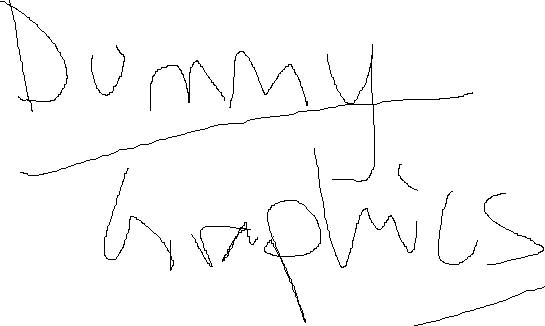
\includegraphics[width=0.85\textwidth]{dummy.png} \label{frq_vs_ampl_plot}
	\caption{Frequency vs. amplitude, before and after corrections. We see a clear relationship between the parameters.}
\end{figure}
The model for correcting the amplitude assumes that real amplitude is linear with apparent amplitude and goes to zero when we set the amplitude like so in software. This model is not perfect, but limitations with our ability to measure one set frequency vs. amplitude for a large number of apparent amplitudes limits us to making assumptions about the system. We see our corrections is a significant improvement to blindly trusting the apparent values. The large error bars primarily comes from the conversion from arbitrary units of acceleration into SI units. 

To get an idea of our baseline noise in measurements, we have collected a dataset comprised solely of noise. Taking the standard derivative will give us a measurement of the typical error. 

Seeing the plots of frequency vs amplitude, one might suspect the natural frequency of the system to be close to 20 Hz. To confirm this suspicion we have conducted two experiments. First, we hit the speaker sharply and measured the acceleration: 
\begin{figure}[h!]
	\centering
	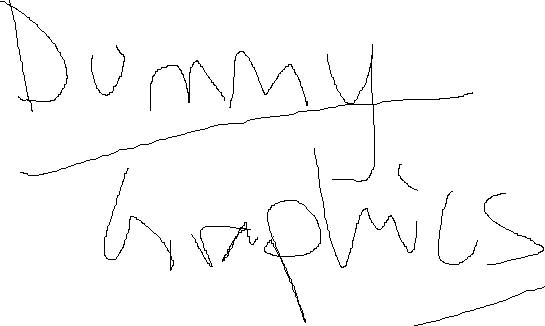
\includegraphics[width=0.85\textwidth]{dummy.png} \label{nat_freq}
	\caption{Ring-out of the speaker membrane after a sharp collision.}
\end{figure}
Assuming this a linearly damped system, we can measure the natural frequency with strong agreement to the earlier shown plot. 

We also measured to real phase of the system and compared it to the apparent phase. The signal used to control the speaker will give us a reference $\pi\cdot N$ phase, which we have compared to the measured phase from accelerometer data. A plot of phaseshift vs frequency looks like:
\begin{figure}[h!]
	\centering
	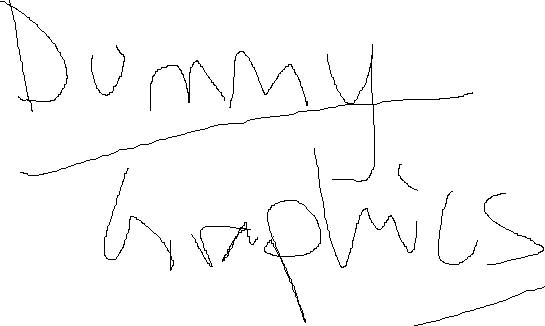
\includegraphics[width=0.85\textwidth]{dummy.png} \label{phaseshift_plot}
	\caption{Phaseshift between the driven frequency and the real frequency.}
\end{figure}
A derivation of the phaseshifts depedency to driven frequency will be given in the appendix. This measurements corroborates our earlier suggestion of the natural frequency being right centered in the frequency domain of interest, suggesting the need for a correction model. 

\subsubsection{The coefficient of restitution}
On very important parameter in the setup is the coefficient of restitution $C_r$ which has already been described in the above. To measure it we used the fact the length of each jump on a plate at rest is proportional to the initial velocity. Since the jump the will be symmetric the initial and final velocity will be equal but with opposite signs. By equation (\ref{flytime}) and setting $\Delta y_k=0$ we can obtain the following ratio, which is exactly $C_r$.
\begin{equation}
	\frac{\Delta t_{k+1}}{\Delta t_{k}}= \frac{\frac{2v_{k+1}}{g}}{\frac{2v_{k}}{g}} = \frac{v_{k+1}}{v_k} = \frac{v_{k+1}}{v_{k,f}} = C_r
\end{equation}

\section{Numerical simulation}
As described in section \ref{modelling} it is not possible to solve the the systems equations of motion analytically in the general case as it require one to find the intersection between a parabola and a sine wave. In the numerical realm it is however possible to find a such intersection. The actual problem is to find where \eqref{platey} and \eqref{ybeq} are equal that is solving the following
\begin{equation}
	A \cos(2\pi f t+ \phi) = -\frac{g}{2}(t-t_k)^2+v_k(t-t_k)+y_p(t_k)
\end{equation}
As described this can easily be done numerically, and the initial velocity for the next jump follows from the equations derived in section \ref{modelling}. 

\subsection{Chaotic behavior in the theoretical model}
The idea for the experiment originates from Tufillaro and Albano\cite{tufillaro}, who suggested that the bouncing ball behaves very much like the quadratic map described in section \ref{chaos}. We however discovered a wide range of chaotic behavior even with a non-chaotic parameter set...

\newpage
\bibliographystyle{plain}
\bibliography{ref}

% % % % % % % % % % % % % % % % % % % % % % Appendix % % % % % % % % % % % % % % % % % % % % % % % % %
\newpage
\appendix
\section{Derivation of the equations of motion for a driven harmonic oscillator}
The equation of motion for a driven simple harmonic oscillator will be of the form:
\begin{align*}
my'' + by' + ky = F\sin(\omega t)\\
y'' + \frac{b}{m}y' + \frac{k}{m} y = F \sin(\omega t)
\end{align*}
We will then write the general solution as a sum of the particular and the homogenues solutions:
\begin{align*}
y_g = y_{h} + y_p
\end{align*}
The homogeneous solution for the damped harmonic oscillator will go to zero with time. We claim it is only the particular solution that matters. To solve this, we will guess the solution to be of the form:
\begin{align*}
y_p = A \sin (\omega t) + B \cos(\omega t)
\end{align*}
We will perform the differentiation and plug into the equation to get:
\begin{align*}
&m\left(-A\omega^2\sin(\omega t) - B\omega^2\cos(\omega t)\right) + b\left(A\omega\cos(\omega t) - B\omega\sin(\omega t)\right) + k\left( A\sin(\omega t) + B\cos(\omega t) \right)\\
&=\sin(\omega t) \left( -mA\omega^2 -bB\omega + kA \right) + \cos(\omega t)\left(-mB\omega^2 + bA\omega + Bk\right)
\end{align*}
After collecting the coefficients, we can match the left side, with the right side:
\begin{align}
F &= -mA\omega^2 -bB\omega + Ak \label{lignA} \\ 
0 &= -mB\omega^2 + bA\omega + Bk \label{lignB}
\end{align}
We isolate an expression for $B$ in (\ref{lignB})
\begin{align*}
B &= \frac{-bA\omega}{-m\omega^2+k}
\end{align*}
Which we will proceed to plug into (\ref{lignA}), to obtain an expression for $A$:
\begin{align*}
A = \frac{F}{-m\omega^2+k+\frac{b^2\omega^2}{-m\omega^2+k}} = \frac{F\left(k-m\omega^2\right)}{\left(k-m\omega^2\right)^2+b^2\omega^2}
\end{align*} 
We can write $A$ and $B$ independently of each other:
\begin{align*}
B &= \frac{-bF\omega}{\left(k-m\omega^2\right)^2+b^2\omega^2}\\
A &=  \frac{F\left(k-m\omega^2\right)}{\left(k-m\omega^2\right)^2+b^2\omega^2}
\end{align*}
We would now like to express $y_p$ in the shape:
\begin{align*}
y_p = L \sin(\omega t + \phi)
\end{align*}
If we write the sine addition identity,
\begin{align*}
L sin(\omega t + \phi) = L\cos(\phi)\sin(\omega t) + L\sin(\phi)\cos(\omega t)
\end{align*}
We see, that our amplitude must obey,
\begin{align*}
A = L\cos(\phi)\\
B = L\sin(\phi)
\end{align*}
if we are to get our initial guess of
\begin{align*}
y_p = A \sin (\omega t) + B \cos(\omega t)
\end{align*}
The phase shift will then be:
\begin{align*}
\frac{B}{A} &= \frac{L\sin(\phi)}{L\cos(\phi)} = \tan(\phi)\\
\phi &= \arctan\left(\frac{B}{A}\right)\\
\phi &= \arctan\left( \frac{-bF\omega}{\left(k-m\omega^2\right)^2+b^2\omega^2} \cdot \frac{\left(k-m\omega^2\right)^2+b^2\omega^2}{F\left(k-m\omega^2\right)} \right)\\
\phi &= \arctan\left( \frac{b\omega}{m\omega^2-k} \right)
\end{align*}
\end{document}
